\documentclass[12pt]{article}
\usepackage{newclude}
\usepackage[utf8]{inputenc}
\usepackage[acronym, toc]{glossaries}
\usepackage{amsmath,amsthm}
\usepackage{amssymb,amsfonts,latexsym,cancel}
\usepackage{graphicx}
\usepackage{float}
\usepackage{subfig}
\usepackage[normalem]{ulem}
\usepackage[lmargin=3cm,rmargin=3cm,top=2.5cm,bottom=2.5cm]{geometry}
\usepackage{longtable}
\usepackage{ragged2e}
\usepackage{datetime}
\usepackage{siunitx}
\usepackage{tikz}
\usetikzlibrary{shapes, positioning}
\usepackage{parskip}
\usepackage{fancyhdr}
\usepackage{titling}
\pagestyle{fancy}
\setlength{\headheight}{15.71667pt}
\usepackage{hyperref}
\hypersetup{
    colorlinks,
    citecolor=black,
    filecolor=black,
    linkcolor=black,
    urlcolor=black
}

\usepackage[
  backend=biber,
  style=ieee,
  url=false,
  doi=true,
  isbn=false
]{biblatex}
\addbibresource{bib/bibliography.bib}

\fancyfoot{}
\renewcommand{\footrulewidth}{0.5pt}
\fancyfoot[R]{\thepage}

\title{ SIFT Algorithm % Título de la práctica
}
\author{ Sergio Marín Sánchez % Nombre del autor
}
\newdate{date}{1}{4}{2024} % Fecha

\begin{document}
\begin{titlepage}
    \centering
    \phantom{a}
    \vspace{2cm}
    {
\includegraphics[scale=0.9]{ESCUDO_UPM.pdf}\par}
    \vspace{2cm}
    {\bfseries\LARGE Universidad Politécnica de Madrid \par}
    \vspace{0.75cm}
    {\scshape\Large Escuela Técnica Superior de Ingenieros Informáticos \par}
    \vspace{0.75cm}
    {\scshape\Huge \thetitle \par}
    \vfill
    {\large Authors: \par}
    {\large \theauthor \par } 
    {\large Álvaro García Barragán  \par }
    {\large Mikel de la Fuente Landa \par }
    \vspace{0.2cm}
    {\large Date: \displaydate{date} \par}
\end{titlepage}

\setcounter{page}{1}

The Scale-Invariant Feature Transform (SIFT) algorithm, is a powerful tool for detecting and describing local features in images, which are robust to changes in scale, rotation, illumination, and viewpoint.

SIFT works by identifying keypoints in an image that are distinctive and repeatable across different images. These keypoints are found by detecting extrema in the scale-space of the image, which means looking for local maxima and minima (Fig. \ref{fig:minima}) in a series of progressively smoothed images, Fig. \ref{fig:smooth}. This scale-space representation allows SIFT to detect keypoints at different scales, enabling robustness to changes in object size and distance from the camera.

\begin{figure}[H]
    \centering
    \subfloat[Smoothing process \cite{huang_high-performance_2012}]{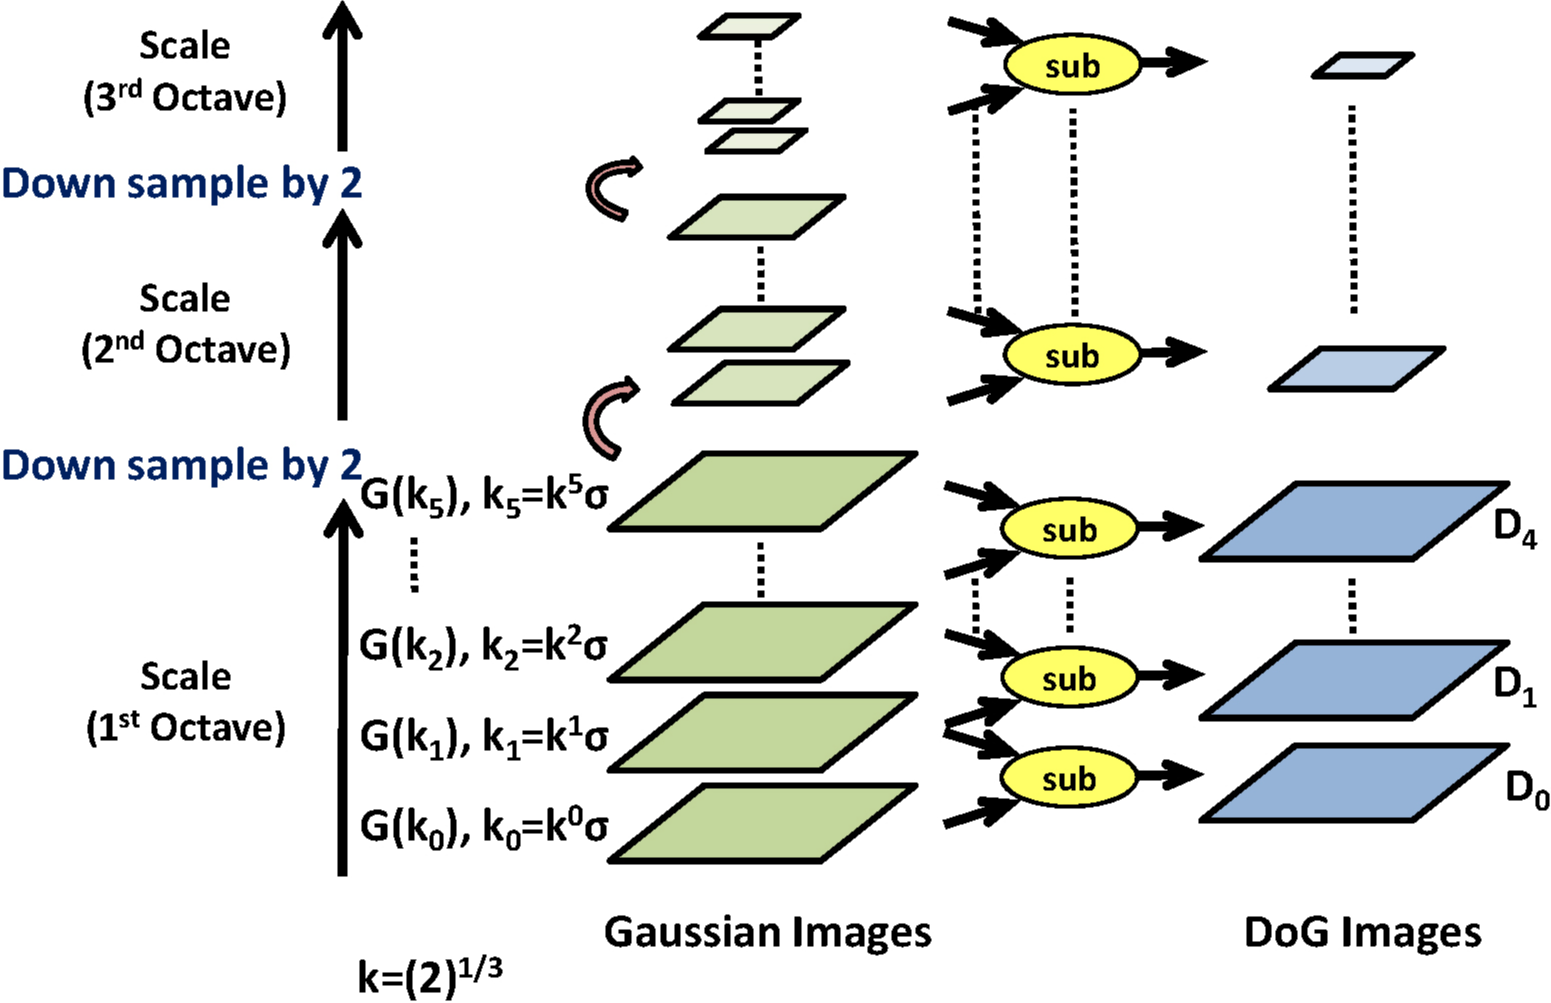
\includegraphics[width=0.5\textwidth]{img/dog.png}\label{fig:smooth}} \quad
    \subfloat[Local minima/maxima \cite{huang_high-performance_2012}]{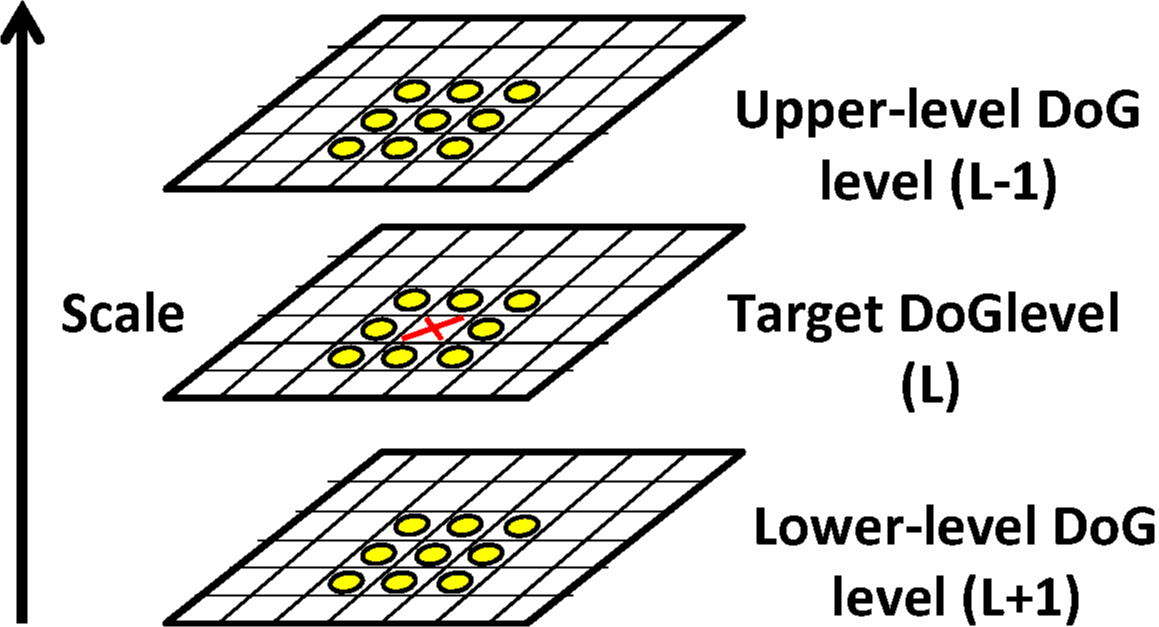
\includegraphics[width=0.4\textwidth]{img/keypoint_detection.png}\label{fig:minima}}
\end{figure}
\setcounter{figure}{1}
\setcounter{subfigure}{0}

Once keypoints are identified, SIFT computes a descriptor for each keypoint, which encodes information about the local image structure around that point. This descriptor is invariant to changes in scale, rotation, and illumination, making it highly distinctive and suitable for matching keypoints across different images. The descriptor is computed based on the gradient orientation histograms of image patches surrounding the keypoint, providing robustness to local geometric transformations. This process is schematized in Fig. \ref{fig:calculation}.

\begin{figure}[H]
    \centering
    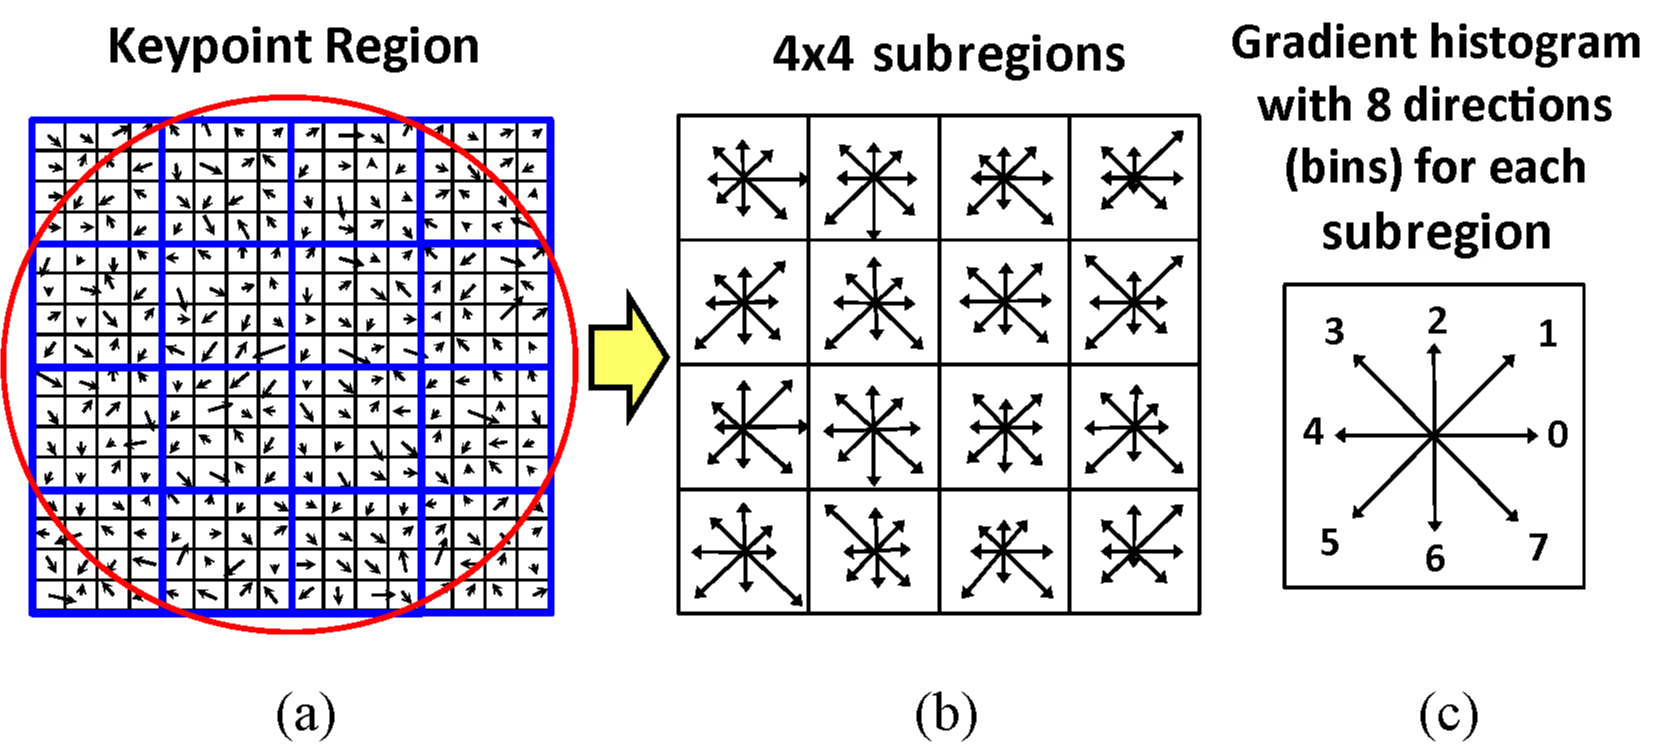
\includegraphics[width=0.8\textwidth]{img/keypoint_calculation.png}
    \caption{Calculation of descriptors \cite{huang_high-performance_2012}}
    \label{fig:calculation}
\end{figure}

\clearpage

Finally, SIFT performs keypoint matching by comparing the descriptors of keypoints between different images. This matching process is typically done using nearest-neighbor search techniques, such as brute-force matching or more efficient methods like kd-trees or approximate nearest neighbors. By matching keypoints based on their descriptors, SIFT enables tasks such as image alignment, object recognition, and image stitching, even in the presence of significant changes in viewpoint or lighting conditions.

It was our task to develop a system that performs SIFT algorithm. We managed to do it and identify objects even when the luminosity has changed (Fig. \ref{fig:results}).

\begin{figure}[H]
    \centering
    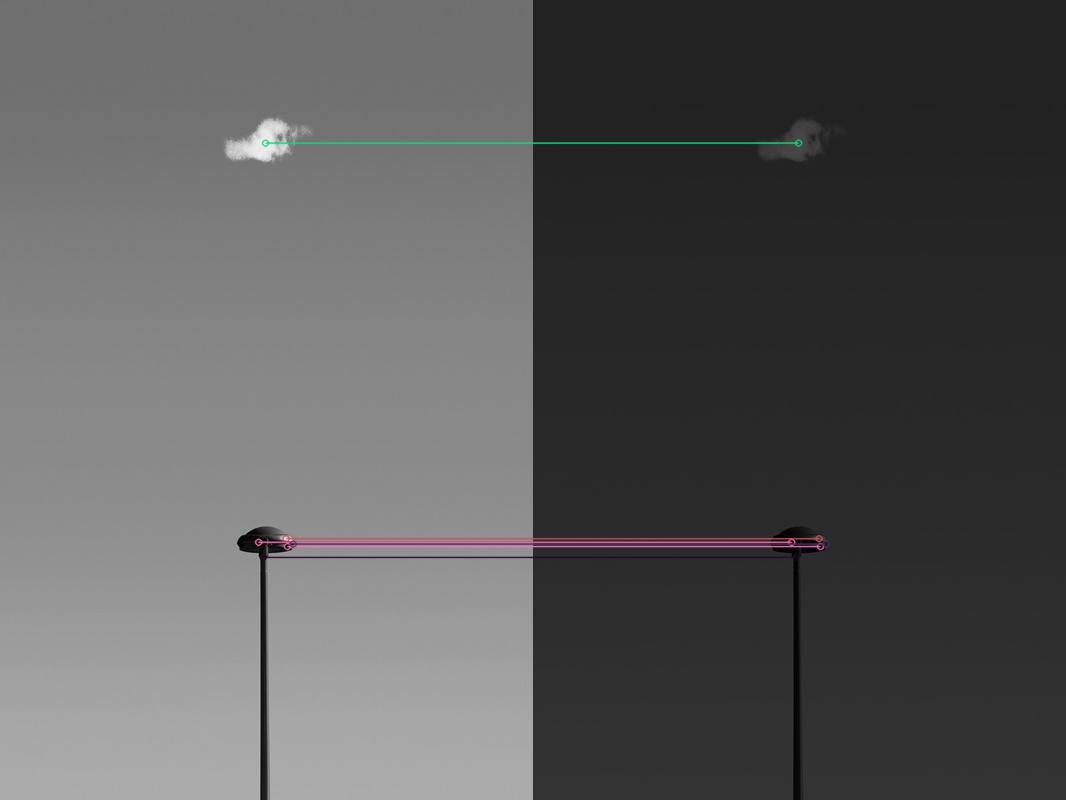
\includegraphics[width=0.8\textwidth]{img/final.png}
    \caption{Results from our implementation}
    \label{fig:results}
\end{figure}

\nocite{*}

\clearpage

\printbibliography

\end{document}
